\documentclass[../../../../main.tex]{subfiles}

\begin{document}

\section*{京大理科数学 1970 表紙・配点・概略}

\begin{itemize}
    \item 所要時間: 40 分 / 150 分
\end{itemize}

\subsection*{難易度・分野一覧}
\begin{enumerate}
    \item 関数 (難易度: A, 計算: A, 思考: A)
    \item 不等式 (難易度: B, 計算: B, 思考: B)
    \item 空間 (難易度: A, 計算: A, 思考: A)
    \item 図形-多変数 (難易度: C, 計算: C, 思考: C)
    \item 関数 (難易度: A, 計算: A, 思考: A)
    \item 数列 (難易度: A, 計算: A, 思考: A)
\end{enumerate}

\subsection*{各問のメモ・解答概要}
\begin{enumerate}
    \item 関数: $g'(a) = 0$
    \item 不等式: (証明)
    \item 空間: (証明)
    \item 図形-多変数: 劣弧 AB の中点, A, B からの距離が各々 $\left( \sqrt{2}l \pm \sqrt{2l^2 - 2r(r - \sqrt{r^2 - l^2})} \right)$ なる優弧 AB 上の 2 点 (計 3 点)
    \item 関数: $x = (2n-1)\pi$ で極大値 $\frac{2}{3}(2n-1)\pi$ ($n \in \mathbb{N}$)
    \item 数列: (イ) (証明), (ロ) (証明), (ハ) $\displaystyle \lim_{n \to \infty} x_n = 1$
\end{enumerate}

\newpage

\section*{第1問}

\noindent
[\textbf{解}] 題意から $y = f'(a)(x-a) + f(a)$ が $(c,0)$ を通る.
\[
0 = f'(a)(c-a) + f(a) \quad \dots \text{①}
\]
又, $g(x)$ の定義から
\[
g'(x) = \frac{f'(x)(x-c) - f(x)}{(x-c)^2}
\]
だから
\[
g'(a) = \frac{f'(a)(a-c) - f(a)}{(a-c)^2} = 0 \quad (\because \text{①}) \quad \mathbin{/\mkern-5mu/}
\]

\newpage

\section*{第2問}

\noindent
[\textbf{解}] $n=2$ の時 $\left(\frac{3}{2}\right)^2 = \frac{9}{4} > 2 = 2!$ から成立. $n=k$ での成立を仮定する時
\[
f_k(x) = (k+1)\log \frac{k+1}{2} - \sum_{i=1}^k \log i
\]
とした時 $f_k(x) > 0$ である ($\because$ 与の同値).
\begin{align*}
f_{k+1}(x) &= (k+2)\log \frac{k+2}{2} - \sum_{i=1}^{k+1} \log i \\
&= f_k(x) + \underbrace{(k+2)\log\frac{k+2}{2} - (k+1)\log\frac{k+1}{2} - \log(k+1)}_{g(k)} \quad \dots \text{①}
\end{align*}

\noindent
ここで, $g(k) > 0$ を示す ($k \in \mathbb{R}$).
\begin{align*}
g'(k) &= \log\frac{k+2}{2} + \frac{k+1}{k+2} - \left[ \log\frac{k+1}{2} + \frac{k}{k+1} \right] - \frac{1}{k+1} \\
&= \log\frac{k+2}{2} - \log\frac{k+1}{2} - \frac{1}{k+2} \\
g''(k) &= \frac{1}{k+2} - \frac{1}{k+1} + \frac{1}{(k+2)^2} \\
&= \frac{-1}{(k+1)(k+2)^2} < 0
\end{align*}
より $g'(k)$ は単調減少. これと $g'(k) = \log\frac{k+2}{k+1} - \frac{1}{k+2} \to 0$ ($k \to \infty$) から $g'(k) > 0$ だから, $g(k)$ は単調増加であり, $k \ge 1$ の時
\[
g(1) = 2\log\frac{3}{2} - \log 2 = 2\log 3 - 3\log 2 = \log\frac{9}{8} > 0
\]
だから $g(k) > 0 \dots \text{②}$.
②と仮定から, ①より, $f_{k+1}(x) > 0$ となり $n=k+1$ でも成立.

\noindent
以上より示された.

\bigskip

\noindent
[\textbf{別 - もっと直接的に示す}]
\begin{align*}
\left(\frac{k+2}{2}\right)^{k+1} - (k+1)! &= \frac{k+2}{2} \left(\frac{k+2}{k+1}\right)^k \left(\frac{k+1}{2}\right)^k - (k+1) \cdot k! \\
&\ge \left[ \frac{k+2}{2} \left(\frac{k+2}{k+1}\right)^k - (k+1) \right] k! \quad (\text{カテイ})
\end{align*}
ここで, $k \ge 2$ のとき, 2項定理から
\[
\left(\frac{k+2}{k+1}\right)^k = \left(1 + \frac{1}{k+1}\right)^k \ge 1 + \frac{k}{k+1} = \frac{2k+1}{k+1}
\]
これから $> 0$ がわかるので OK!! \hfill $\mathbin{/\mkern-5mu/}$

\newpage

\section*{第3問}

\noindent
[\textbf{解}] $l, g$ の単位方向ベクトルを $\vec{l}, \vec{g}$ とする. 又 点 $X$ の位置ベクトルをその小文字で表す. $\alpha, \beta$ を実数として ($0 < \alpha < \beta$)
\begin{align*}
\vec{a_2} &= \vec{a_1} + \alpha \vec{l} \\
\vec{a_3} &= \vec{a_1} + \beta \vec{l} \\
\vec{b_2} &= \vec{b_1} + \alpha \vec{g} \\
\vec{b_3} &= \vec{b_1} + \beta \vec{g}
\end{align*}
とかけるから
\begin{align*}
\vec{m_2} &= \frac{\vec{a_1} + \vec{b_1}}{2} + \frac{\alpha}{2}(\vec{l} + \vec{g}) \\
\vec{m_1} &= \frac{\vec{a_1} + \vec{b_1}}{2} \\
\vec{m_3} &= \frac{\vec{a_1} + \vec{b_1}}{2} + \frac{\beta}{2}(\vec{l} + \vec{g})
\end{align*}
となる. つまり $M_1, M_2, M_3$ は方向ベクトル $\vec{l} + \vec{g}$ とし, $M_1$ を通る直線上にある.

\begin{center}
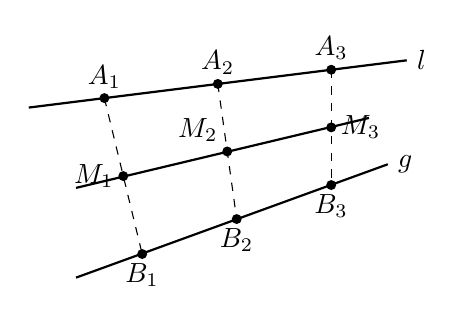
\begin{tikzpicture}[scale=1.2, >=stealth]
  \draw[thick] (0, 2) -- (4, 2.5) node[right] {$l$};
  \draw[thick] (0.5, 0.2) -- (3.8, 1.4) node[right] {$g$};

  \coordinate (A1) at (0.8, 2.1);
  \coordinate (A2) at (2.0, 2.25);
  \coordinate (A3) at (3.2, 2.4);

  \fill (A1) circle (1.5pt) node[above] {$A_1$};
  \fill (A2) circle (1.5pt) node[above] {$A_2$};
  \fill (A3) circle (1.5pt) node[above] {$A_3$};

  \coordinate (B1) at (1.2, 0.45);
  \coordinate (B2) at (2.2, 0.82);
  \coordinate (B3) at (3.2, 1.18);

  \fill (B1) circle (1.5pt) node[below] {$B_1$};
  \fill (B2) circle (1.5pt) node[below] {$B_2$};
  \fill (B3) circle (1.5pt) node[below] {$B_3$};

  \draw[dashed] (A1) -- (B1);
  \draw[dashed] (A2) -- (B2);
  \draw[dashed] (A3) -- (B3);

  \coordinate (M1) at (1.0, 1.275);
  \coordinate (M2) at (2.1, 1.535);
  \coordinate (M3) at (3.2, 1.79);

  \fill (M1) circle (1.5pt) node[left] {$M_1$};
  \fill (M2) circle (1.5pt) node[above left] {$M_2$};
  \fill (M3) circle (1.5pt) node[right] {$M_3$};

  \draw[thick] (0.5, 1.15) -- (3.6, 1.89);
\end{tikzpicture}
\end{center}

\newpage

\section*{第4問}

\noindent
[\textbf{解}] $\angle AOB = \alpha, AP = x, BP = y$ とする ($r \ge l$). 又, $\angle PAB = \beta, \angle PBA = \delta$ とおく.

\bigskip

\noindent
\textbf{1° $P$ が劣弧 AB 上}

\begin{center}
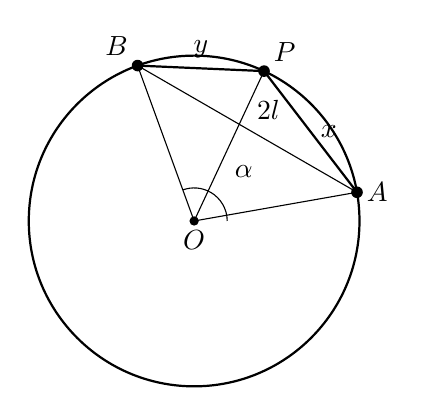
\begin{tikzpicture}[scale=1.4, >=stealth]
  \draw[thick] (0,0) circle (1.5);
  \fill (0,0) circle (1.2pt) node[below] {$O$};

  \coordinate (A) at (10:1.5);
  \coordinate (B) at (110:1.5);
  \coordinate (P) at (65:1.5);

  \fill (A) circle (1.5pt) node[right] {$A$};
  \fill (B) circle (1.5pt) node[above left] {$B$};
  \fill (P) circle (1.5pt) node[above right] {$P$};

  \draw (0,0) -- (A);
  \draw (0,0) -- (B);
  \draw (A) -- (B) node[midway, above right] {$2l$};

  \draw[thick] (P) -- (A) node[midway, right] {$x$};
  \draw[thick] (P) -- (B) node[midway, above] {$y$};

  \draw (0,0) -- (P);
  \draw (0.3,0) arc (0:110:0.3);
  \node at (0.45, 0.45) {$\alpha$};
\end{tikzpicture}
\end{center}

\noindent
$\triangle ABP$ に余弦定理を用いて
\[
4l^2 = x^2 + y^2 - 2xy \cos\left(\pi - \frac{\alpha}{2}\right) \quad \dots \text{①}
\]
又, 正弦定理を用いて
\[
\frac{2l}{\sin\left(\pi - \frac{\alpha}{2}\right)} = \frac{y}{\sin\beta} = \frac{x}{\sin\delta} = 2r \quad \dots \text{②}
\]
① に $xy = 2r\left(r - \sqrt{r^2 - l^2}\right)$ を代入,
\begin{align*}
(x+y)^2 &= 4l^2 - 2xy \cos\frac{\alpha}{2} + 2xy \\
&= 4l^2 + 4r\left(r - \sqrt{r^2 - l^2}\right)\left(1 - \cos\frac{\alpha}{2}\right) \quad \dots \text{③}
\end{align*}
又 ② と $0 < \frac{\alpha}{2} \le \frac{\pi}{2}$ から $\cos\frac{\alpha}{2} = \sqrt{1 - \left(\frac{l}{r}\right)^2}$ だから ③ に代入
\begin{align*}
(x+y)^2 &= 4l^2 + 4\left(r - \sqrt{r^2 - l^2}\right)^2 \\
&= 4\left[ l^2 + r^2 + r^2 - l^2 - 2r\sqrt{r^2 - l^2} \right] \\
&= 8\left(r^2 - r\sqrt{r^2 - l^2}\right)
\end{align*}
\[
x+y = \sqrt{8r\left(r - \sqrt{r^2 - l^2}\right)} \quad \dots \text{④}
\]
④ と題意から $t = r - \sqrt{r^2 - l^2}$ とおくと, $x, y$ は $P$ の2次式
\[
t^2 - 2\sqrt{2rt} + 2rt = 0
\]
の2解で
\[
x = y = \sqrt{2rt}
\]
より, $P$ は弧 AB の中点である.

\bigskip

\noindent
\textbf{2° $P$ が優弧 AB 上}

\begin{center}
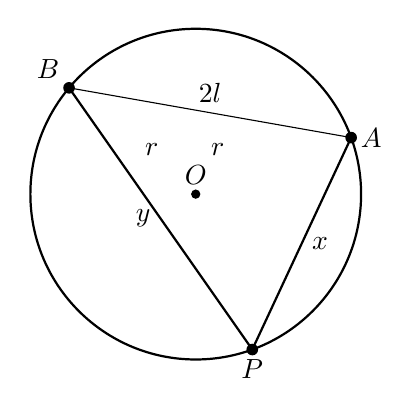
\begin{tikzpicture}[scale=1.4, >=stealth]
  \draw[thick] (0,0) circle (1.5);
  \fill (0,0) circle (1.2pt) node[above] {$O$};

  \coordinate (A) at (20:1.5);
  \coordinate (B) at (140:1.5);
  \coordinate (P) at (-70:1.5);

  \fill (A) circle (1.5pt) node[right] {$A$};
  \fill (B) circle (1.5pt) node[above left] {$B$};
  \fill (P) circle (1.5pt) node[below] {$P$};

  \draw (A) -- (B) node[midway, above] {$2l$};
  \draw[thick] (P) -- (A) node[midway, right] {$x$};
  \draw[thick] (P) -- (B) node[midway, left] {$y$};

  \node at (0.2, 0.4) {$r$};
  \node at (-0.4, 0.4) {$r$};
\end{tikzpicture}
\end{center}

\noindent
$\triangle ABP$ に正弦, 余弦定理を用いて
\begin{align*}
4l^2 &= x^2 + y^2 - 2xy \cos\frac{\alpha}{2} \quad \dots \text{①} \\
\frac{2l}{\sin\frac{\alpha}{2}} &= 2r \quad \dots \text{⑥}
\end{align*}
⑥ と $0 < \frac{\alpha}{2} \le \frac{\pi}{2}$ から $\cos\frac{\alpha}{2} = \sqrt{1 - \left(\frac{l}{r}\right)^2}$. だから ① に代入
\begin{align*}
(x+y)^2 &= 4l^2 + 2xy \cos\frac{\alpha}{2} + 2xy \\
&= 4l^2 + 4r\left(r - \sqrt{r^2 - l^2}\right)\left(1 + \sqrt{1 - \left(\frac{l}{r}\right)^2}\right) \\
&= 4l^2 + 4\left(r^2 - (r^2 - l^2)\right) \\
&= 8l^2
\end{align*}
\[
\therefore x + y = 2\sqrt{2}l
\]
従つて, $x, y$ は $P$ の2次式
\[
P^2 - 2\sqrt{2}l P + 2rt = 0
\]
の2解で
\[
P = \sqrt{2}l \pm \sqrt{2l^2 - 2r\left(r - \sqrt{r^2 - l^2}\right)}
\]
だから, A, B からの距離が各々 $\left( \sqrt{2}l \pm \sqrt{2l^2 - 2r\left(r - \sqrt{r^2 - l^2}\right)} \right)$ なる 2 点.
$P = A$ または $P = B$ の時は $AP \cdot BP = 0$ となるが, この時 $l = 0$ となり不適.

\bigskip

\noindent
以上 1°, 2° から, もとめるのは

劣弧 AB の中点, A, B からの距離が各々 $\left( \sqrt{2}l \pm \sqrt{2l^2 - 2r\left(r - \sqrt{r^2 - l^2}\right)} \right)$ なる優弧 AB 上の 2 点 (計 3 点) である. \hfill $\mathbin{/\mkern-5mu/}$

\newpage

\section*{第5問}

\noindent
[\textbf{解}] $F'(x) = x \sin^3 x$, $0 < x$ から, $\sin x$ の正負をかんがえて

$F'(x)$ は $x = (2n-1)\pi$ ($n \in \mathbb{N}$) の前後で 正から負へと符号がかわり, 他の値でこのやうに変化することはないので $F(x)$ は $x = (2n-1)\pi$ で極大である.

\begin{align*}
F(x) &= \frac{1}{4} \int_0^x t (3\sin t - \sin 3t) \, dt \\
&= \frac{1}{4} \left[ \left( -3t\cos t + 3\sin t \right) - \left( -\frac{1}{3}t\cos 3t + \frac{\sin 3t}{9} \right) \right]_0^x \\
&= \frac{1}{4} \left[ -3x\cos x + 3\sin x + \frac{1}{3}x\cos 3x - \frac{1}{9}\sin 3x \right]
\end{align*}
より
\begin{align*}
F((2n-1)\pi) &= \frac{1}{4} \left[ +3(2n-1)\pi + \frac{1}{3}(2n-1)\pi (-1) \right] \\
&= \frac{2}{3}(2n-1)\pi \quad (n \in \mathbb{N}) \quad \mathbin{/\mkern-5mu/}
\end{align*}

\newpage

\section*{第6問}

\noindent
[\textbf{解}] (イ) 帰納法で示す. $n=2$ の時 成立. $n=k$ での成立を仮定すると
\begin{align*}
x_{k+1} &= \frac{x_k^2 + 2}{3} > \frac{1+2}{3} = 1 \\
x_{k+1} &< \frac{a^2 + 2}{3} < a \quad (\because a^2 - 3a + 2 = (a-2)(a-1) < 0)
\end{align*}
より $n=k+1$ でも成立. 以上から示された.

\bigskip

\noindent
(ロ)
\begin{align*}
|x_{n+1} - 1| &= \frac{1}{3}(x_n^2 + 2) - 1 = \frac{1}{3}(x_n + 1)(x_n - 1) \\
&< \frac{1}{3}(a + 1)(x_n - 1) \quad (\because (\text{イ}))
\end{align*}

\bigskip

\noindent
(ハ) くり返し用いて
\[
0 < x_n - 1 \le \left(\frac{a+1}{3}\right)^{n-1}(a - 1)
\]
よつて はさみうちから $\displaystyle x_n \to 1 \ (n \to \infty)$ \hfill $\mathbin{/\mkern-5mu/}

\end{document}
